Natural language processing relies on almost all computer science fundamental, specially statistics and Neural Networks.

This chapter focuses on the required mathematics and computer science which are used in further chapters from the paper.

\section{Bayes Theorem}

Bayes theorem describes the probability of an event, based on prior knowledge of conditions that might be related to the event.
$$ P(A \mid B) = \frac{P(B \mid A) \, P(A)}{P(B)} $$


\section{Text representation And language modeling}

Words belong to a set of semi-structured data known as language, which contains information about itself.
One way to view language is as a form of data compression, in which knowledge of the world is consolidated into a symbolic set.

But text in it's raw form doesn't represent any knowledge or feature for any algorithm, thus to be able to apply any advanced algorithms that works on a contextual level of the text we first needs text analysis and information retrieval methods to be able to represent that contextual knowledge.

Therefore, we need to re-format the text into feature vectors to be able to represent the context and knowledge within the text.

\vspace{.5cm}

\subsection{Word embedding}

Natural language processing systems traditionally treat words as discrete atomic symbols, and therefore 'cat' may be represented as Id537 and 'dog' as Id143. This encoding is arbitrary, and provide no useful information to the system regarding the relationships that may exist between the individual symbols. This means that the model can leverage very little of what it has learned about 'cats' when it is processing data about 'dogs' (such that they are both animals, four-legged, pets, etc.). Representing words as unique, discrete ids furthermore leads to data sparsity, and usually means that we may need more data in order to successfully train statistical models. Using vector representations can overcome some of these obstacles.

Vector space models (VSMs) represent (embed) words in a continuous vector space where semantically similar words are mapped to nearby points ('are embedded nearby each other'). VSMs have a long, rich history in NLP, but all methods depend in some way or another on the Distributional Hypothesis, which states that words that appear in the same contexts share semantic meaning.

\subsection{Word2Vec}

Word2Vec is a method to efficiently create word embeddings and has been around since 2013. Word2Vec is a two-layer neural net that processes text. Its input is a text corpus and its output is a set of vectors: feature vectors for words in that corpus. While Word2Vec is not a deep neural network, it turns text into a numerical form that deep nets can understand.

\begin{figure}[ht]
    \centering
    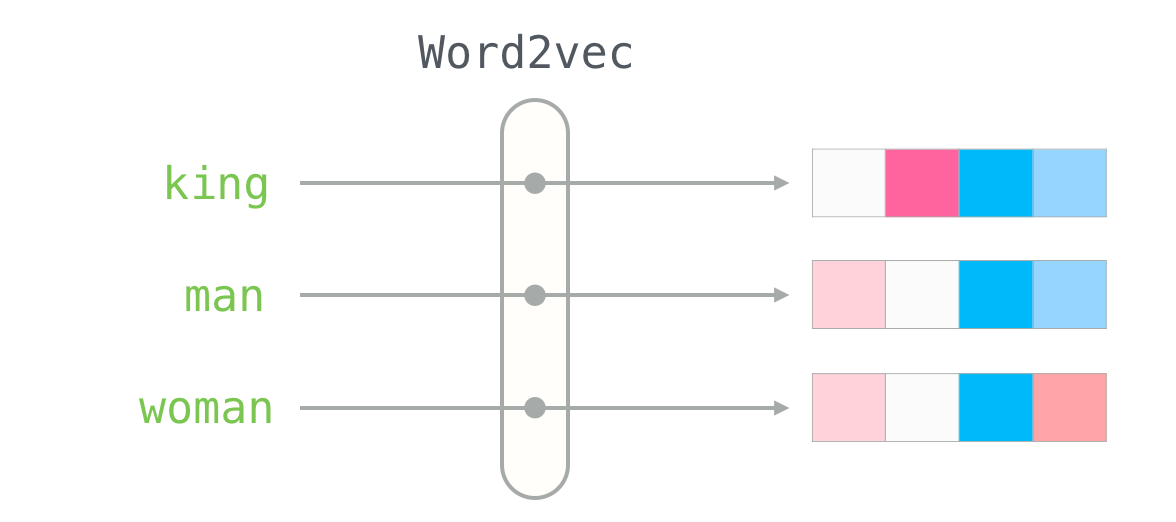
\includegraphics[scale=0.3]{Images/word2vec.png}
    \caption{Word2Vec Illustration}
    \label{fig:w2v}
\end{figure}

\vspace{3cm}

\subsection{Pre-trained Word2Vec}
Building a word2vec model require a very large language corpus with billions of words and sentences. Thus, Using a pre-trained word2vec is a very common practice in NLP.

Previously, we mentioned \textbf{Vector Space Models (VSMs)}, VSMs represents words as set of vectors. These vectors are used in the mathematical and statistical models for classification and regression tasks. Also, they shall be unique to be able to distinguish between them when they are proceeded to the other models.

Training a Word2Vec is the process of building a \textbf{Shallow Neural Network} that for a given word in the middle of a sentence (the input word), look at the words nearby and pick one at random. The network is going to tell us the probability for every word in our vocabulary of being the “nearby word” that we chose.


\begin{figure}[ht]
    \centering
    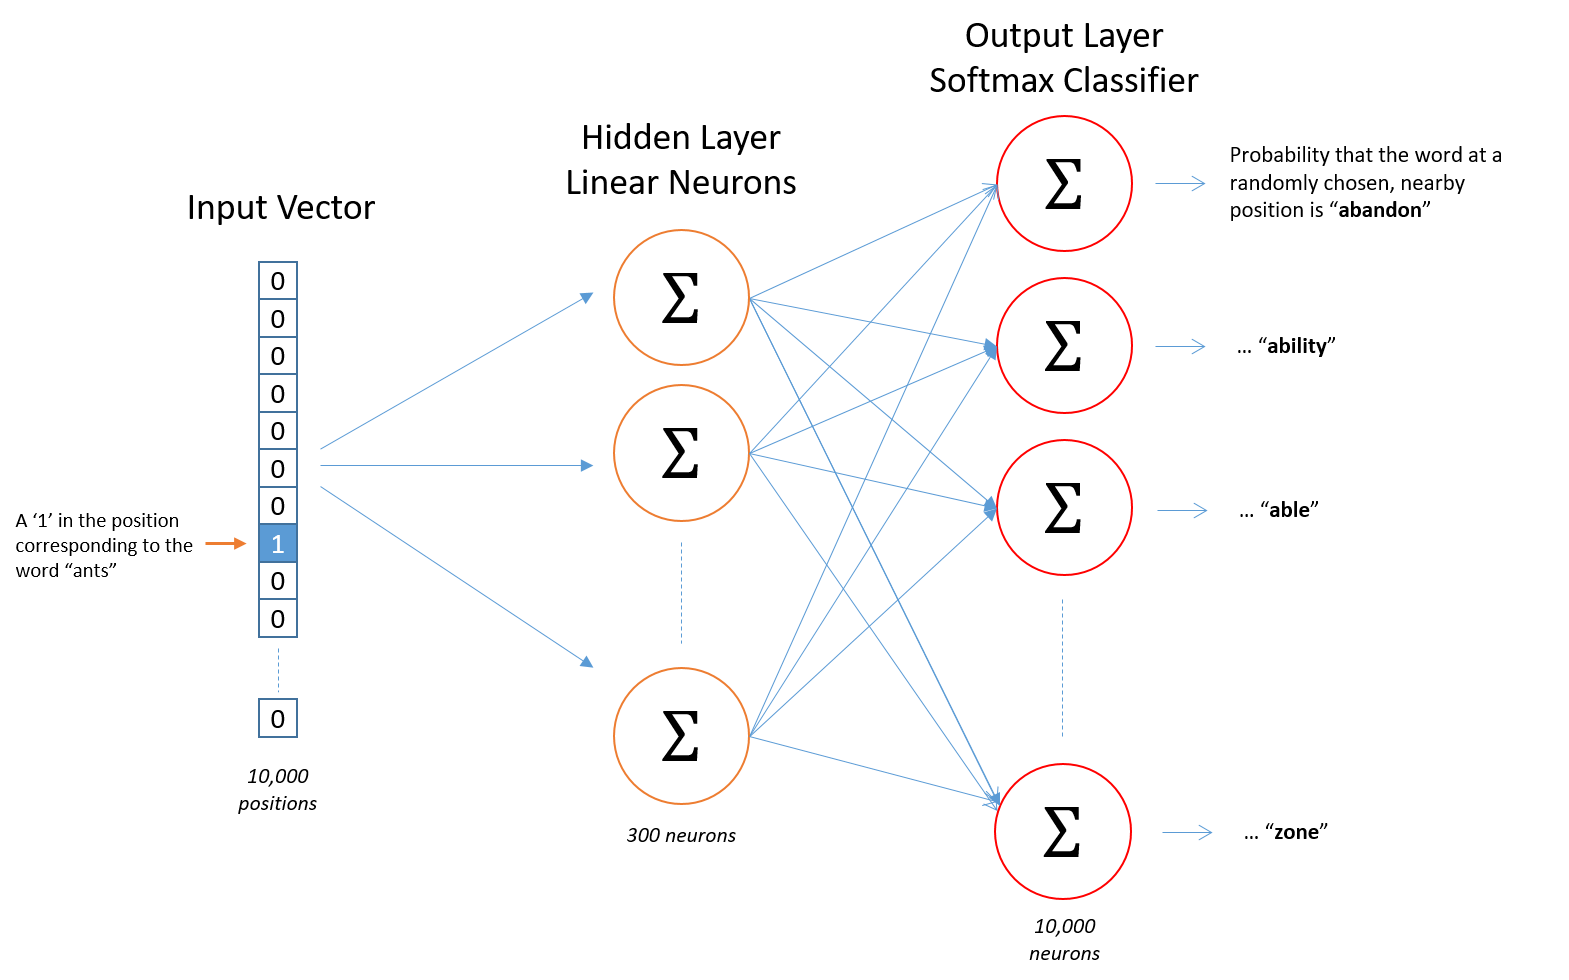
\includegraphics[scale=0.3]{Images/word2vec-shallow-network.png}
    \caption{Word2Vec shallow network Architecture}
    \label{fig:w2vsnas}
\end{figure}





\subsection{Bag-of-words}

Bag of words (BOW) is an algorithm that counts how many times a word appears in a document. It’s a tally. Those word counts allow us to compare documents and gauge their similarities for applications like search, document classification and topic modeling. BOW is a also method for preparing text for input in a deep-learning neural networks.

\begin{table}[ht]
\centering
\caption{Bag of words}
\begin{tabular}{|l|l|l|l|} 
\hline
Word & Doc 1 & Doc 2 & Doc 3  \\ 
\hline
Car  & 4     & 2     & 7      \\ 
\hline
Boy  & 3     & 1     & 5      \\ 
\hline
Park & 3     & 6     & 2      \\
\hline
\end{tabular}
\end{table}

All the vectors get normalized before getting fed to any algorithm. Thus, the frequency of each word is effectively converted to represent the probabilities of those words’ occurrence in the document


\subsection{Continuous Bag of Words}
 
 In the continuous bag of words model, context is represented by multiple words for a given target words. For example, we could use “cat” and “tree” as context words for “climbed” as the target word.
 
 The CBOW model architecture tries to predict the current target word (the center word) based on the source context words (surrounding words). Considering a simple sentence, “the quick brown fox jumps over the lazy dog”, this can be pairs of (\textit{context window, target word}) where if we consider a context window of size 2, we have examples like ([quick, fox], brown), ([the, brown], quick), ([the, dog], lazy) and so on. Thus the model tries to predict the \textit{target word} based on the \textit{context window} words.
 

\subsection{Skip-gram}

The Skip-gram model architecture usually tries to achieve the reverse of what the CBOW model does. It tries to predict the source context words (surrounding words) given a target word (the center word). Considering our simple sentence from earlier, “the quick brown fox jumps over the lazy dog”. If we used the CBOW model, we get pairs of (\textit{context window, target word})where if we consider a context window of size 2, we have examples like \textit{([quick, fox], brown), ([the, brown], quick), ([the, dog], lazy)} and so on. Now considering that the skip-gram model’s aim is to predict the context from the target word, the model typically inverts the contexts and targets, and tries to predict each context word from its target word. Hence the task becomes to predict the context \textit{[quick, fox]} given target word \textit{‘brown’} or \textit{[the, brown]} given target word ‘quick’ and so on. Thus the model tries to predict the context window words based on the target word.


\begin{figure}[ht]
    \centering
    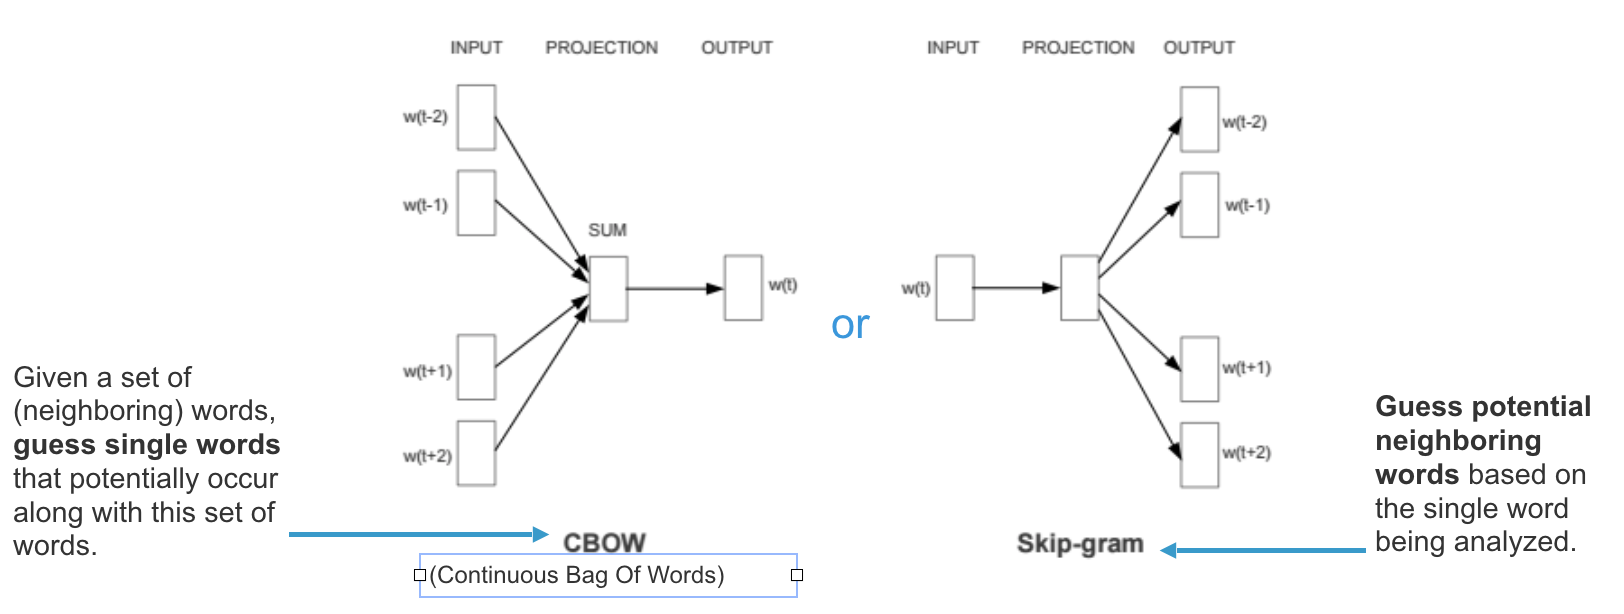
\includegraphics[scale=0.3]{Images/cbow-sg.png}
    \caption{CBOW vs Skip-gram for word2vec}
    \label{fig:cbowsg}
\end{figure}



\subsection{Hierarchical Softmax}

Hierarchical softmax is an alternative to the softmax in which the probability of any one outcome depends on a number of model parameters that is only logarithmic in the total number of outcomes. In “vanilla” softmax, on the other hand, the number of such parameters is linear in the number of total number of outcomes.
The consequence is that models using hierarchical softmax are significantly faster to train with stochastic gradient descent, since only the parameters upon which the current training example depend need to be updated, and less updates means we can move on to the next training example sooner. At evaluation time, hierarchical softmax models allow faster calculation of individual outcomes, again because they depend on less parameters (and because the calculation using the parameters is just as straightforward as in the softmax case.

\vspace{1 cm}

In general, the target of Softmax layer is to maximize the probability of a word given its context P(word | context). Assume that from our dataset and using CBOW model, we want to predict the word “unseen” given the context “The”, “blade” and “is”. So, our probability formula would be P(unseen | the, blade, is).

Regularly, we use a flat Softmax layer to get that probability after applying the Softmax formula and get the probabilities. But in Hierarchical Softmax we don’t use a flat layer, but instead, we use a balanced Huffman tree layer \\

\vspace{1 cm}

Recalling softmax, we can view the softmax method as a tree where the root node is the hidden layer activation (or context vector ��), and the leaves are the probabilities of each word.

\begin{figure}[ht]
    \centering
    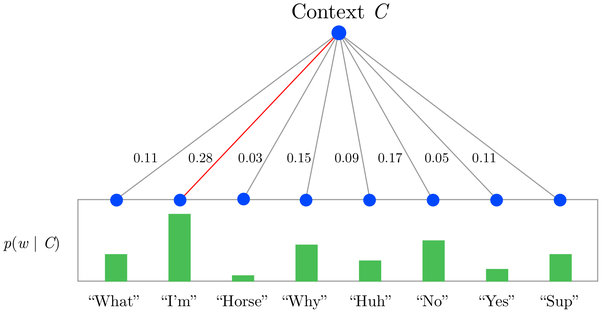
\includegraphics[scale=0.7]{Images/hsmx.png}
    \caption{Softmax as a tree}
    \label{fig:smxtree}
\end{figure}

Note that to find the probability of a given word, you must compute all of the terminal leaves.

A hierarchical softmax instead computes the values of the leaves with a multi-layer tree.

\begin{figure}[ht]
    \centering
    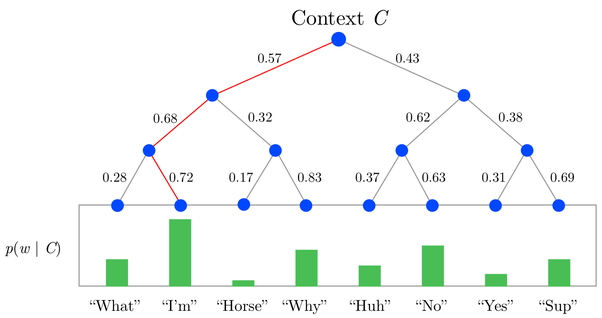
\includegraphics[scale=0.7]{Images/hsmx2.png}
    \caption{Hierarchical Softmax as a tree}
    \label{fig:smxtree}
\end{figure}

To evaluate the probability of a given word, take the product of the probabilities of each edge on the path to that node:

P(I'm|C)=0.57∗0.68∗0.72=0.28

Now, in the case of a binary tree, this can provide an exponential speedup. In the case of 1 million words, the computation involves log(1000000)=20 multiplications!


\section{Recurrent Neural Networks}
\subsection{RNN}

Recurrent nets are a type of artificial neural network designed to recognize patterns in sequences of data, such as text, genomes, handwriting, These algorithms take time and sequence into account, they have a temporal dimension.

RNNs address the problem of context by using memory units. The output that the RNN produce at step is affected by the output from the step. So in general RNN has two sources of input. One is the actual input and two is the context (memory) unit from previous input.

\begin{figure}[ht]
    \centering
    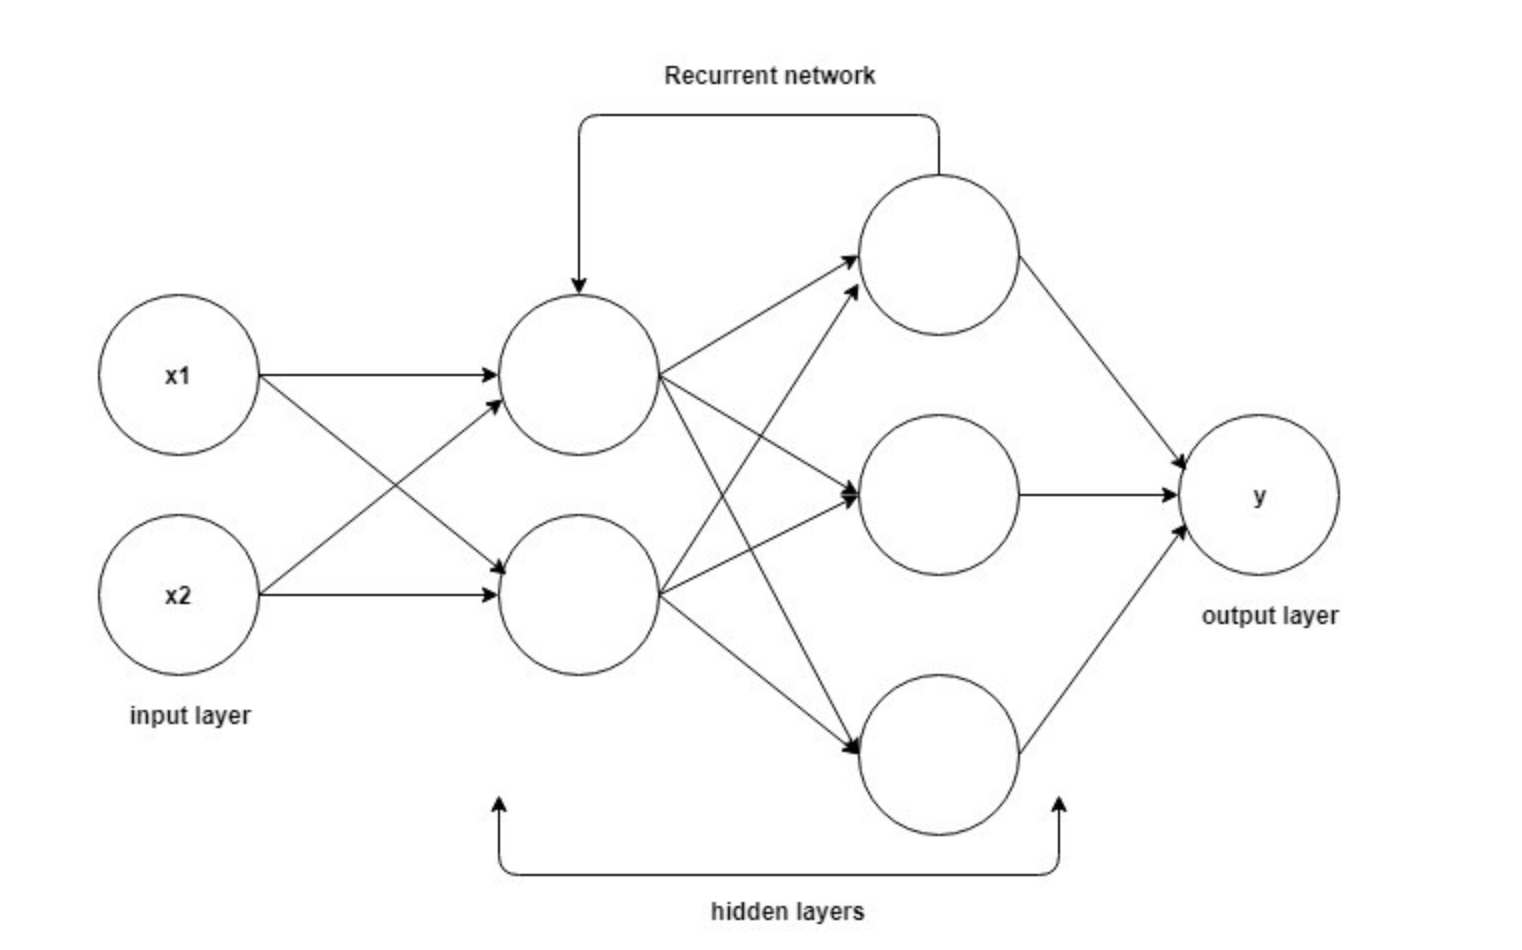
\includegraphics[scale=0.3]{Images/recurrent-nets.png}
    \caption{RNN Illustration}
    \label{fig:rnnI}
\end{figure}

\subsection{LSTM unit}

Long short-term memory units is a special type of Recurrent neural network. The only difference between RNN and LSTM that instead of having a single neural network layer in RNN. We have 4 NN layers in LSTM interacting together.

The core of a cell state is the horizontal line that connects between and. This line is where the data flow happens to throw the chain of the cell states. It’s very easy for the data to flow with minimum linear operations or unchanged this whole process is controlled by Gates.
Gates are what control the change of the data. They change the data optionally with a sigmoid neural layer and a vector multiplication operation.

The Sigmoid layer is a method that generates float value between and this value control how much data will be passed through the gate. means nothing while one means all.
The first step is that the sigmoid layer decides what information to pass from the result of multiplying by. We can represent this operation mathematically like this:

The previous step did decide what data it’ll forget and what data it’ll carry on. In the second step, we need to actually do this.
We take the previous result and multiply it by the old state.
The old state is computed using the Tanh activation function. Multiplying the sigmoid by the tanh will decide which information the network forget and which get. Mathematically:
Finally, we need to decide what is the value of the output is
Those operations are applied sequentially on the chain of cell states.

\begin{figure}[ht]
    \centering
    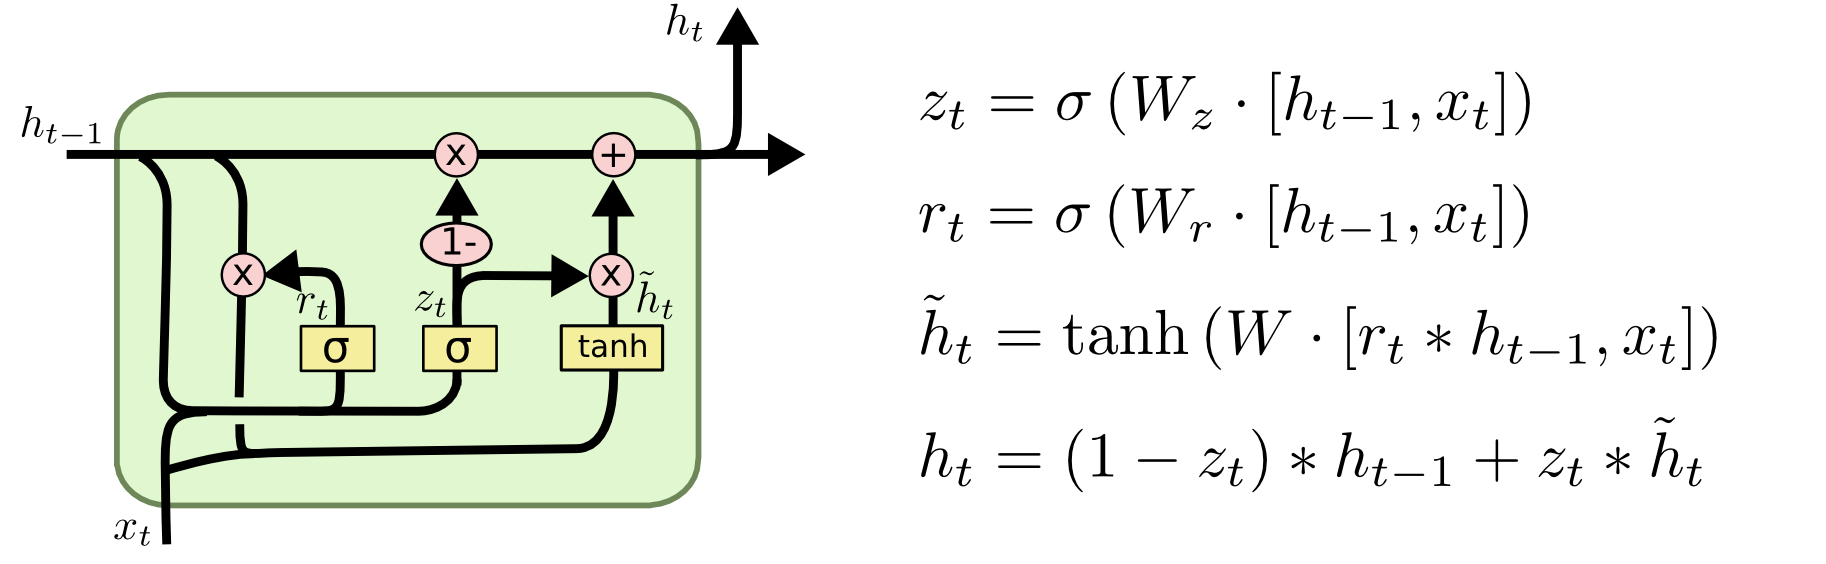
\includegraphics[scale=0.7]{Images/LSTM3-var-GRU.png}
    \caption{LSTM Unit illustration}
    \label{fig:lstm}
\end{figure}

Usually, Complex models, uses a method called stacking LSTM to deal with complex contextual data like Arabic language
